\subsection{Result analysis}\label{Subsec:results}
The results of each test will in this section be compared to the baseline RMSE as seen in \autoref{fig:base_errors}, and with the RMSE score of the different methods.


\begin{figure}[H]
	\centering
	\begin{adjustbox}{width=0.5\textwidth}
		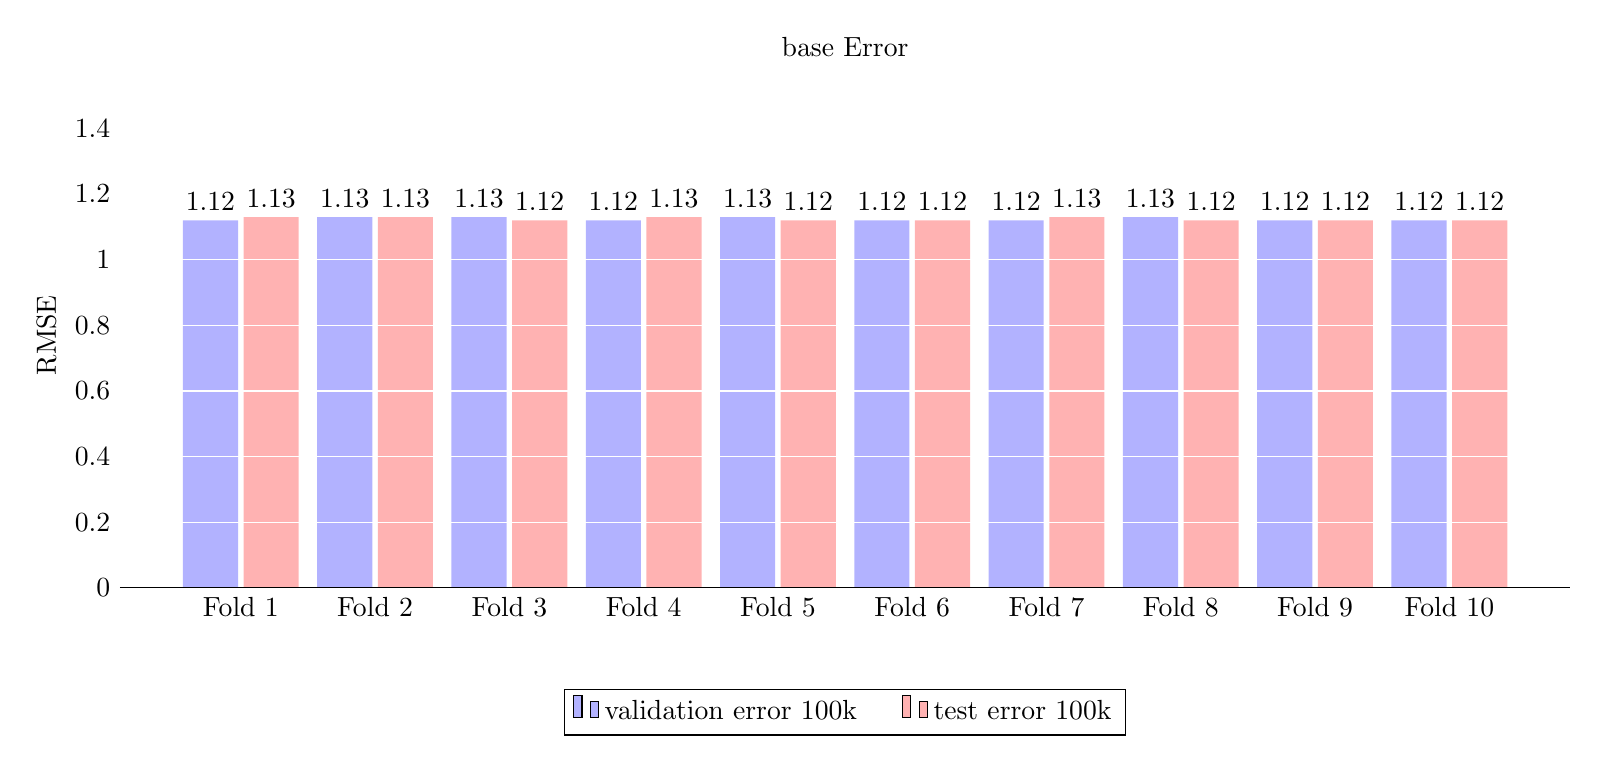
\begin{tikzpicture}
  \centering
  \begin{axis}[
        ybar, axis on top,
        title={base Error},
        height=8cm, width=20cm,
        bar width=0.7cm,
        ymajorgrids, tick align=inside,
        major grid style={draw=white},
        enlarge y limits={value=.1,upper},
        ymin=0, ymax=1.4,
        axis x line*=bottom,
        y axis line style={opacity=0},
        tickwidth=0pt,
        enlarge x limits=true,
        legend style={
            at={(0.5,-0.2)},
            anchor=north,
            legend columns=-1,
            /tikz/every even column/.append style={column sep=0.5cm}
        },
        ylabel={RMSE},
        symbolic x coords={
           Fold 1,Fold 2,
           Fold 3,Fold 4,
           Fold 5,Fold 6,
           Fold 7,Fold 8,
           Fold 9,Fold 10},
       xtick=data,
       nodes near coords={
        \pgfmathprintnumber[precision=2]{\pgfplotspointmeta}
       }
    ]
    \addplot [draw=none, fill=blue!30] coordinates {
      (Fold 1, 1.12)
      (Fold 2, 1.13)
      (Fold 3, 1.13)
      (Fold 4, 1.12)
      (Fold 5, 1.13)
      (Fold 6, 1.12)
      (Fold 7, 1.12)
      (Fold 8, 1.13)
      (Fold 9, 1.12)
      (Fold 10, 1.12)};
   \addplot [draw=none,fill=red!30] coordinates {
      (Fold 1, 1.13)
      (Fold 2, 1.13)
      (Fold 3, 1.12)
      (Fold 4, 1.13)
      (Fold 5, 1.12)
      (Fold 6, 1.12)
      (Fold 7, 1.13)
      (Fold 8, 1.12)
      (Fold 9, 1.12)
      (Fold 10, 1.12)};
    \legend{validation error 100k, test error 100k}
  \end{axis}
\end{tikzpicture}
	\end{adjustbox}
	\caption{base error from 100k dataset }
	\label{fig:base_errors}
\end{figure}

In \autoref{fig:base_errors} we have the baseline RMSE, we got this by using the average rating for the dataset as the prediction for all future ratings.

\begin{figure}[H]
	\centering
	\begin{adjustbox}{width=0.5\textwidth}
		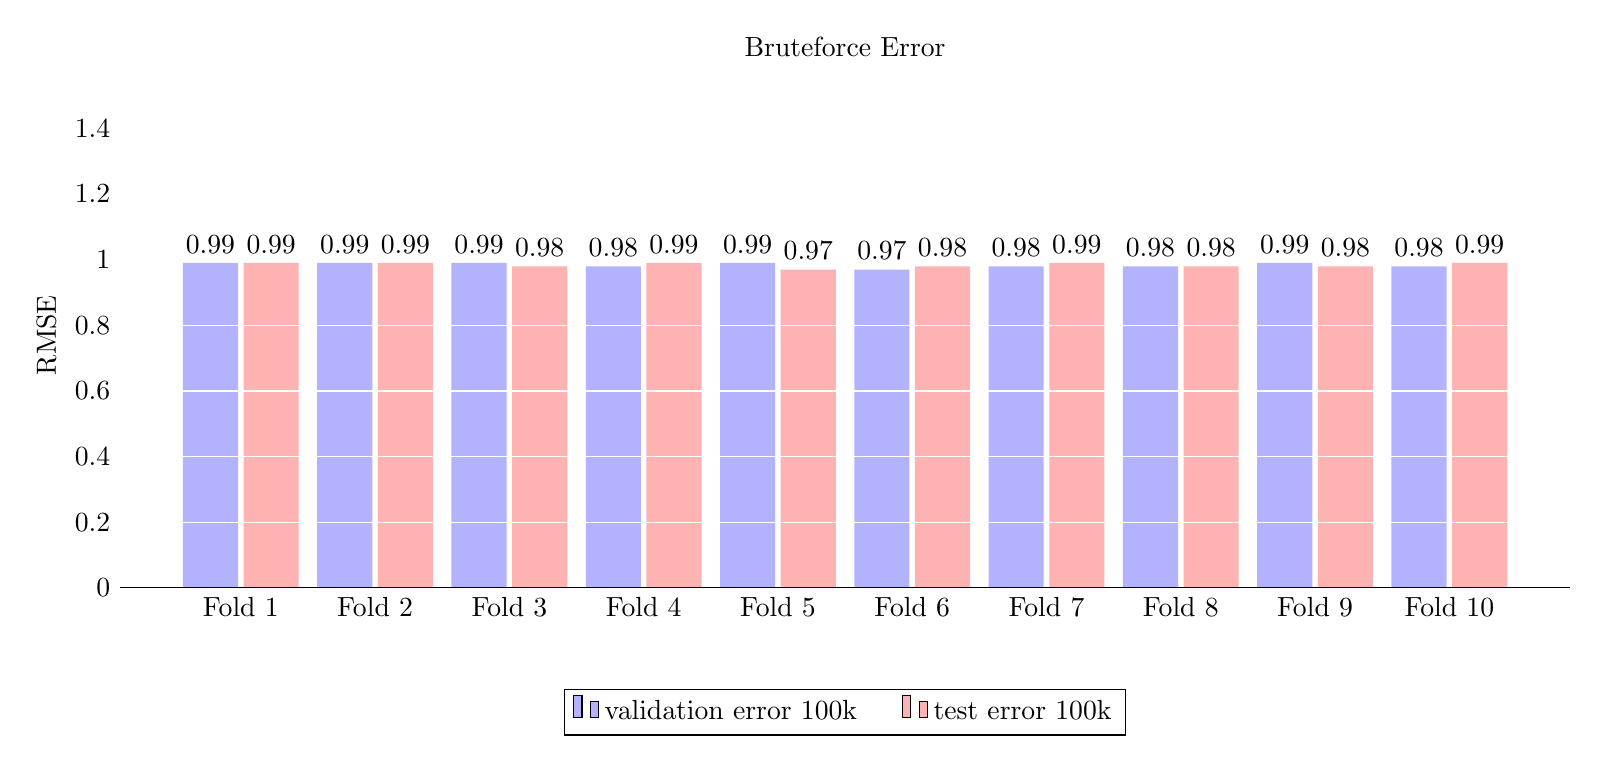
\begin{tikzpicture}
  \centering
  \begin{axis}[
        ybar, axis on top,
        title={Bruteforce Error},
        height=8cm, width=20cm,
        bar width=0.7cm,
        ymajorgrids, tick align=inside,
        major grid style={draw=white},
        enlarge y limits={value=.1,upper},
        ymin=0, ymax=1.4,
        axis x line*=bottom,
        y axis line style={opacity=0},
        tickwidth=0pt,
        enlarge x limits=true,
        legend style={
            at={(0.5,-0.2)},
            anchor=north,
            legend columns=-1,
            /tikz/every even column/.append style={column sep=0.5cm}
        },
        ylabel={RMSE},
        symbolic x coords={
           Fold 1,Fold 2,
           Fold 3,Fold 4,
           Fold 5,Fold 6,
           Fold 7,Fold 8,
           Fold 9,Fold 10},
       xtick=data,
       nodes near coords={
        \pgfmathprintnumber[precision=2]{\pgfplotspointmeta}
       }
    ]
    \addplot [draw=none, fill=blue!30] coordinates {
      (Fold 1, 0.99)
      (Fold 2, 0.99)
      (Fold 3, 0.99)
      (Fold 4, 0.98)
      (Fold 5, 0.99)
      (Fold 6, 0.97)
      (Fold 7, 0.98)
      (Fold 8, 0.98)
      (Fold 9, 0.99)
      (Fold 10, 0.98)};
   \addplot [draw=none,fill=red!30] coordinates {
      (Fold 1, 0.99)
      (Fold 2, 0.99)
      (Fold 3, 0.98)
      (Fold 4, 0.99)
      (Fold 5, 0.97)
      (Fold 6, 0.98)
      (Fold 7, 0.99)
      (Fold 8, 0.98)
      (Fold 9, 0.98)
      (Fold 10, 0.99)};
    \legend{validation error 100k, test error 100k}
  \end{axis}
  \end{tikzpicture}
	\end{adjustbox}
	\caption{bruteforce error from 100k dataset }
	\label{fig:brute_errors}
\end{figure}

\autoref{fig:brute_errors} show the RMSE for the 20 evaluations. 
This shows that with a relatively simple method, recommendations can be done better than the baseline.
\autoref{fig:brute_errors} also shows that the RMSE in most folds only have a difference of $0.01$ between validation and test sets.

\begin{figure}[H]
	\centering
	\begin{adjustbox}{width=0.5\textwidth}
		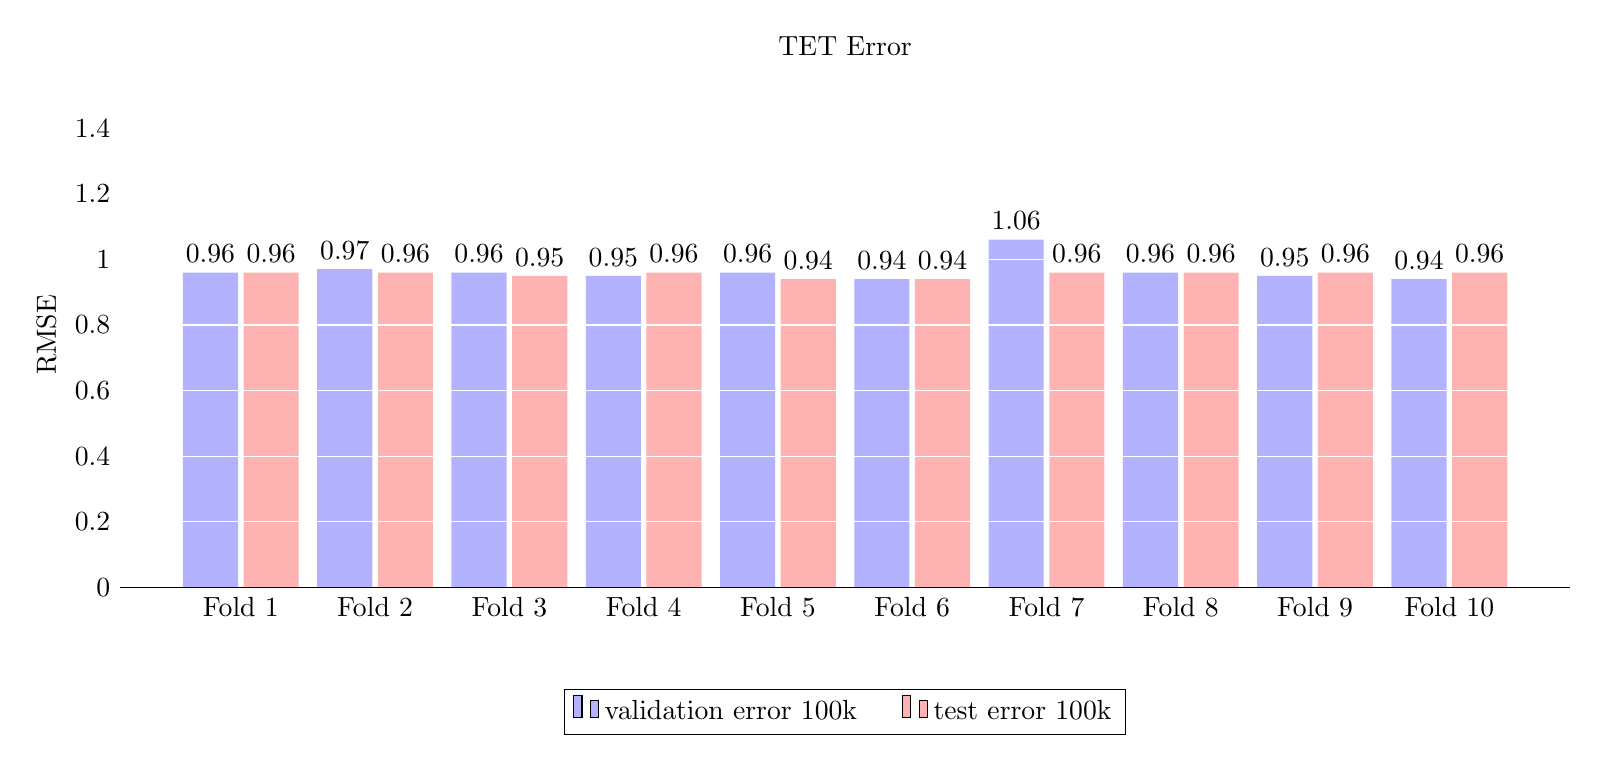
\begin{tikzpicture}
  \centering
  \begin{axis}[
        ybar, axis on top,
        title={TET Error},
        height=8cm, width=20cm,
        bar width=0.7cm,
        ymajorgrids, tick align=inside,
        major grid style={draw=white},
        enlarge y limits={value=.1,upper},
        ymin=0, ymax=1.4,
        axis x line*=bottom,
        y axis line style={opacity=0},
        tickwidth=0pt,
        enlarge x limits=true,
        legend style={
            at={(0.5,-0.2)},
            anchor=north,
            legend columns=-1,
            /tikz/every even column/.append style={column sep=0.5cm}
        },
        ylabel={RMSE},
        symbolic x coords={
           Fold 1,Fold 2,
           Fold 3,Fold 4,
           Fold 5,Fold 6,
           Fold 7,Fold 8,
           Fold 9,Fold 10},
       xtick=data,
       nodes near coords={
        \pgfmathprintnumber[precision=2]{\pgfplotspointmeta}
       }
    ]
    \addplot [draw=none, fill=blue!30] coordinates {
      (Fold 1, 0.96)
      (Fold 2, 0.97)
      (Fold 3, 0.96)
      (Fold 4, 0.95)
      (Fold 5, 0.96)
      (Fold 6, 0.94)
      (Fold 7, 1.06)
      (Fold 8, 0.96)
      (Fold 9, 0.95)
      (Fold 10, 0.94)};
   \addplot [draw=none,fill=red!30] coordinates {
      (Fold 1, 0.96)
      (Fold 2, 0.96)
      (Fold 3, 0.95)
      (Fold 4, 0.96)
      (Fold 5, 0.94)
      (Fold 6, 0.94)
      (Fold 7, 0.96)
      (Fold 8, 0.96)
      (Fold 9, 0.96)
      (Fold 10, 0.96)};
    \legend{validation error 100k, test error 100k}
  \end{axis}
  \end{tikzpicture}
	\end{adjustbox}
	\caption{Node2vec error from 100k dataset}
	\label{fig:N2V_errors}
\end{figure}

The graph in \autoref{fig:N2V_errors} shows the most promising of our results with RMSE values being as low as 0.94 . By tweaking the metadata of the training we believe that there are potential for even better recommendations.
The discrepancy between validation and test in fold 7 seems to indicate that this fold has been fitted wrongly.


\begin{figure}[H]
	\centering
	\begin{adjustbox}{width=0.5\textwidth}
		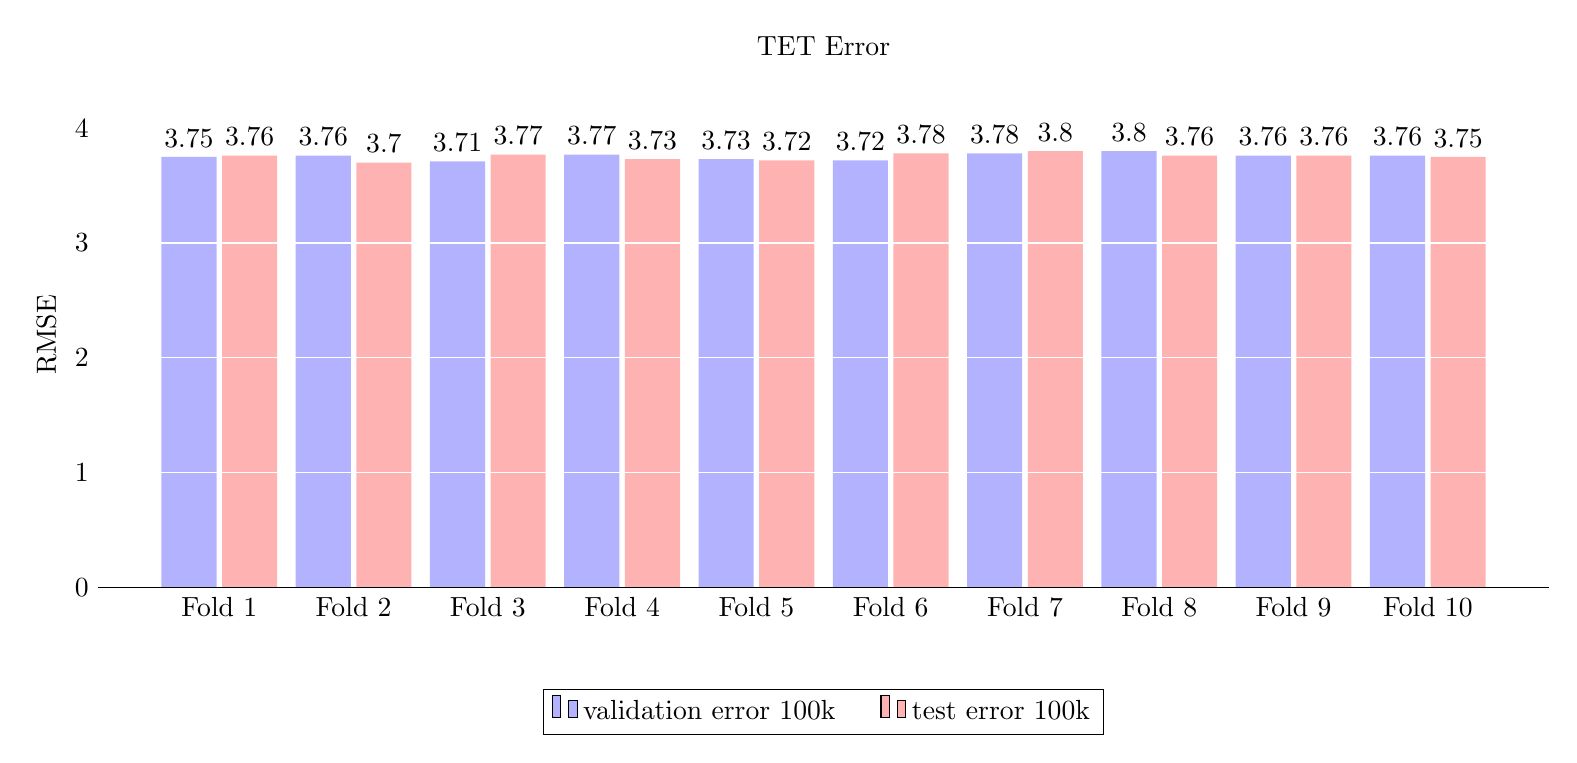
\begin{tikzpicture}
  \centering
  \begin{axis}[
        ybar, axis on top,
        title={TET Error},
        height=8cm, width=20cm,
        bar width=0.7cm,
        ymajorgrids, tick align=inside,
        major grid style={draw=white},
        enlarge y limits={value=.1,upper},
        ymin=0, ymax=4,
        axis x line*=bottom,
        y axis line style={opacity=0},
        tickwidth=0pt,
        enlarge x limits=true,
        legend style={
            at={(0.5,-0.2)},
            anchor=north,
            legend columns=-1,
            /tikz/every even column/.append style={column sep=0.5cm}
        },
        ylabel={RMSE},
        symbolic x coords={
           Fold 1,Fold 2,
           Fold 3,Fold 4,
           Fold 5,Fold 6,
           Fold 7,Fold 8,
           Fold 9,Fold 10},
       xtick=data,
       nodes near coords={
        \pgfmathprintnumber[precision=2]{\pgfplotspointmeta}
       }
    ]
    \addplot [draw=none, fill=blue!30] coordinates {
      (Fold 1, 3.75)
      (Fold 2, 3.76)
      (Fold 3, 3.71)
      (Fold 4, 3.77)
      (Fold 5, 3.73)
      (Fold 6, 3.72)
      (Fold 7, 3.78)
      (Fold 8, 3.80)
      (Fold 9, 3.76)
      (Fold 10, 3.76)};
   \addplot [draw=none,fill=red!30] coordinates {
      (Fold 1, 3.76)
      (Fold 2, 3.70)
      (Fold 3, 3.77)
      (Fold 4, 3.73)
      (Fold 5, 3.72)
      (Fold 6, 3.78)
      (Fold 7, 3.80)
      (Fold 8, 3.76)
      (Fold 9, 3.76)
      (Fold 10, 3.75)};
%   \addplot [draw=none, fill=green!30] coordinates {
%      (Sep-11,75.4064)
%      (Oct-11, 89.7961) 
%      (Nov-11,94.4597)
%      (Dec-11,76.6786) 
%      (Jan-12,77.5600) 
%      (Feb-12,78.2339)
%      (Mar-12,88.6138) 
%      (Apr-12,78.9129) };

    \legend{validation error 100k, test error 100k}
  \end{axis}
  \end{tikzpicture}
	\end{adjustbox}
	\caption{TET error from 100k dataset }
	\label{fig:tet_errors}
\end{figure}


The RMSE scores for the TETs seen in \autoref{fig:tet_errors}, are at a glance not impressive, but the RMSE scores are still better than the baseline.

This shows potential in the framework and it might be better with more descriptive features. The advantage of recommendation with TETs, is that it can depend only on structural information.
Where the other methods we have discussed are dependent on the nearest neighbors having rated a product or movie to make a recommendation, the TETs only need movies or products that look like the movie or product you try to predict a recommendation for.

A scenario where the TETs structure should be better is with the addition of new items in the database.
We made this scenario by removing any relation to all the movies in the verification and test sets from all users in the traning set.
As a consequence, we do not have their input to the prediction.
We ran the scenario on the TETs and Node2vec.

\begin{figure}[H]
	\centering
	\begin{adjustbox}{width=0.5\textwidth}
		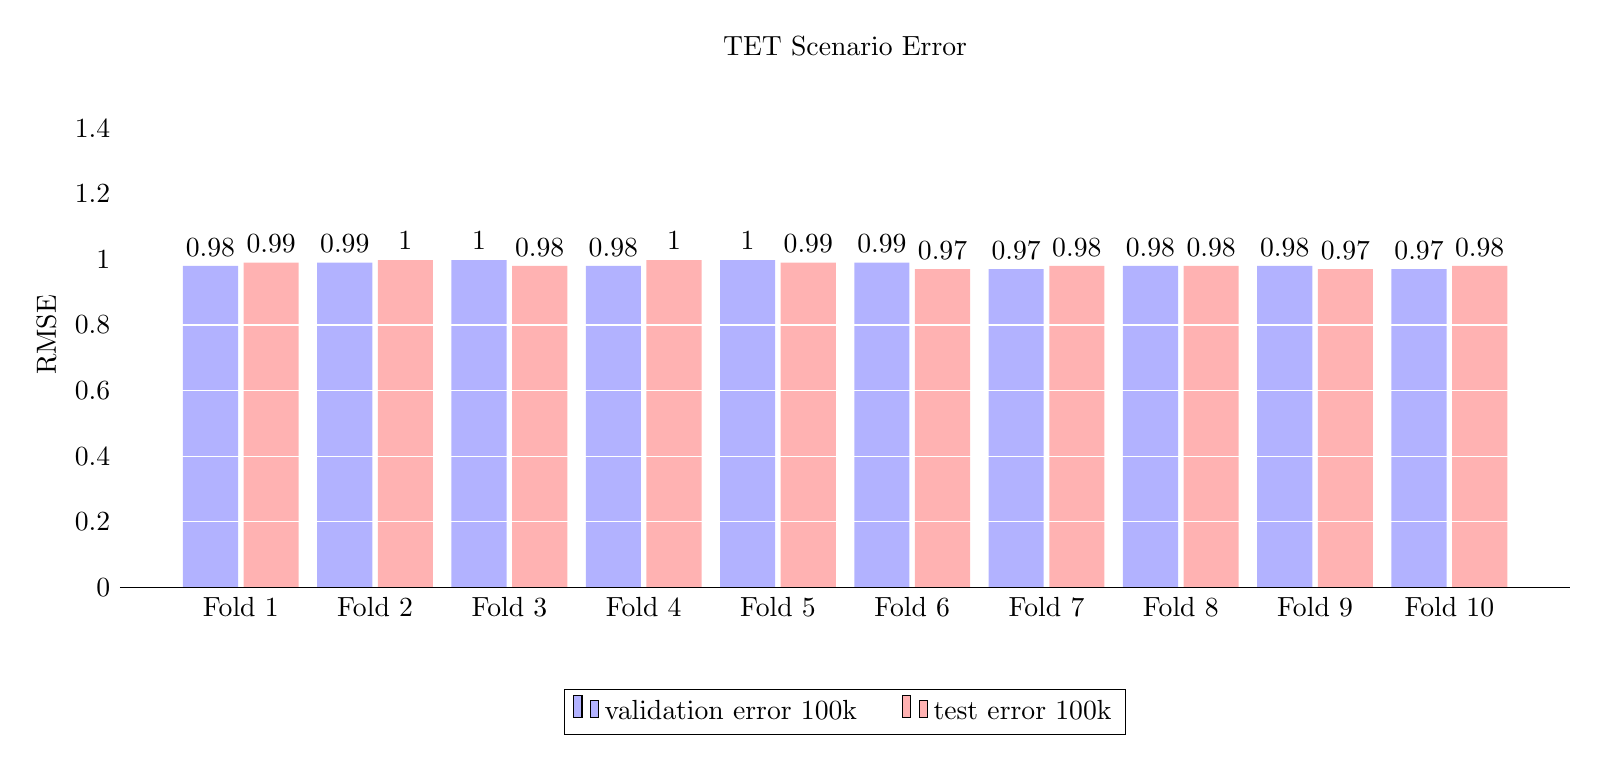
\begin{tikzpicture}
  \centering
  \begin{axis}[
        ybar, axis on top,
        title={TET Scenario Error},
        height=8cm, width=20cm,
        bar width=0.7cm,
        ymajorgrids, tick align=inside,
        major grid style={draw=white},
        enlarge y limits={value=.1,upper},
        ymin=0, ymax=1.4,
        axis x line*=bottom,
        y axis line style={opacity=0},
        tickwidth=0pt,
        enlarge x limits=true,
        legend style={
            at={(0.5,-0.2)},
            anchor=north,
            legend columns=-1,
            /tikz/every even column/.append style={column sep=0.5cm}
        },
        ylabel={RMSE},
        symbolic x coords={
           Fold 1,Fold 2,
           Fold 3,Fold 4,
           Fold 5,Fold 6,
           Fold 7,Fold 8,
           Fold 9,Fold 10},
       xtick=data,
       nodes near coords={
        \pgfmathprintnumber[precision=2]{\pgfplotspointmeta}
       }
    ]
    \addplot [draw=none, fill=blue!30] coordinates {
      (Fold 1, 0.98)
      (Fold 2, 0.99)
      (Fold 3, 1.00)
      (Fold 4, 0.98)
      (Fold 5, 1.00)
      (Fold 6, 0.99)
      (Fold 7, 0.97)
      (Fold 8, 0.98)
      (Fold 9, 0.98)
      (Fold 10, 0.97)};
   \addplot [draw=none,fill=red!30] coordinates {
      (Fold 1, 0.99)
      (Fold 2, 1.00)
      (Fold 3, 0.98)
      (Fold 4, 1.00)
      (Fold 5, 0.99)
      (Fold 6, 0.97)
      (Fold 7, 0.98)
      (Fold 8, 0.98)
      (Fold 9, 0.97)
      (Fold 10, 0.98)};
    \legend{validation error 100k, test error 100k}
  \end{axis}
\end{tikzpicture}
	\end{adjustbox}
	\caption{abstract baseline error from 100k dataset}
	\label{fig:abstract_baseline_errors}
\end{figure}

Because the TET rating set is split in 3 instead of 5, when making recommendation based on subTETs we are able to recommend within this set.
We abstracted the ratings to this form for the baseline as seen in \autoref{fig:abstract_baseline_errors}.

\begin{figure}[H]
	\centering
	\begin{adjustbox}{width=0.5\textwidth}
		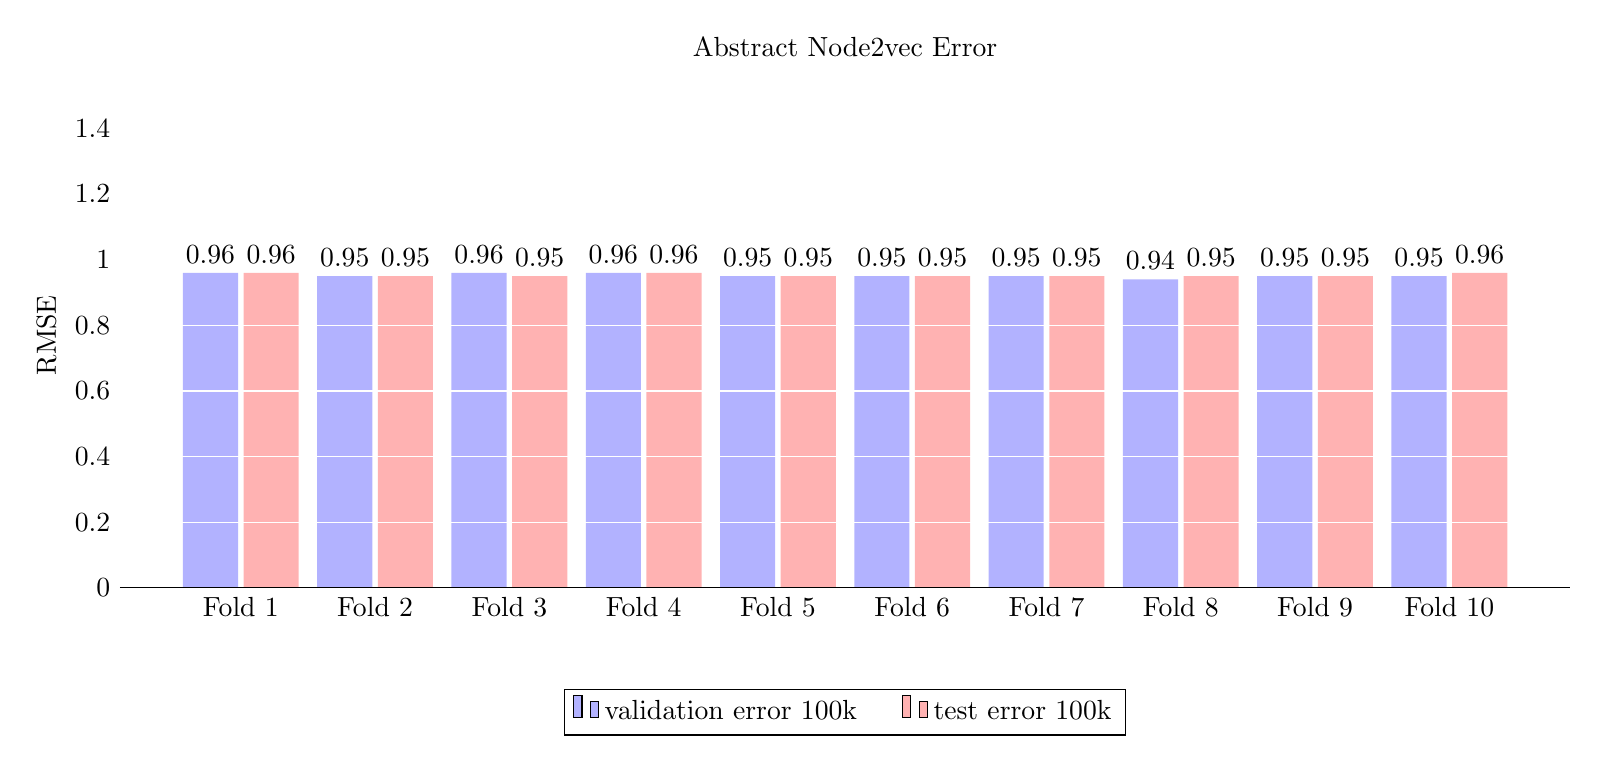
\begin{tikzpicture}
  \centering
  \begin{axis}[
        ybar, axis on top,
        title={Abstract Node2vec Error},
        height=8cm, width=20cm,
        bar width=0.7cm,
        ymajorgrids, tick align=inside,
        major grid style={draw=white},
        enlarge y limits={value=.1,upper},
        ymin=0, ymax=1.4,
        axis x line*=bottom,
        y axis line style={opacity=0},
        tickwidth=0pt,
        enlarge x limits=true,
        legend style={
            at={(0.5,-0.2)},
            anchor=north,
            legend columns=-1,
            /tikz/every even column/.append style={column sep=0.5cm}
        },
        ylabel={RMSE},
        symbolic x coords={
           Fold 1,Fold 2,
           Fold 3,Fold 4,
           Fold 5,Fold 6,
           Fold 7,Fold 8,
           Fold 9,Fold 10},
       xtick=data,
       nodes near coords={
        \pgfmathprintnumber[precision=2]{\pgfplotspointmeta}
       }
    ]
    \addplot [draw=none, fill=blue!30] coordinates {
      (Fold 1, 0.96)
      (Fold 2, 0.95)
      (Fold 3, 0.96)
      (Fold 4, 0.96)
      (Fold 5, 0.95)
      (Fold 6, 0.95)
      (Fold 7, 0.95)
      (Fold 8, 0.94)
      (Fold 9, 0.95)
      (Fold 10, 0.95)};
   \addplot [draw=none,fill=red!30] coordinates {
      (Fold 1, 0.96)
      (Fold 2, 0.95)
      (Fold 3, 0.95)
      (Fold 4, 0.96)
      (Fold 5, 0.95)
      (Fold 6, 0.95)
      (Fold 7, 0.95)
      (Fold 8, 0.95)
      (Fold 9, 0.95)
      (Fold 10, 0.96)};
    \legend{validation error 100k, test error 100k}
  \end{axis}
\end{tikzpicture}
	\end{adjustbox}
	\caption{Node2vec scenario error from 100k dataset}
	\label{fig:N2V_scenario_errors}
\end{figure}

The predictions from node2vec default to the users' average rating since there are no other users that have rated the movies.
When the predictions are calculated they are abstracted similarly to the baseline the RMSE can be seen in \autoref{fig:N2V_scenario_errors}. 
These predictions are still better than baseline because they consider the user's average rating rather than the datasets' average rating.

\begin{figure}[H]
	\centering
	\begin{adjustbox}{width=0.5\textwidth}
		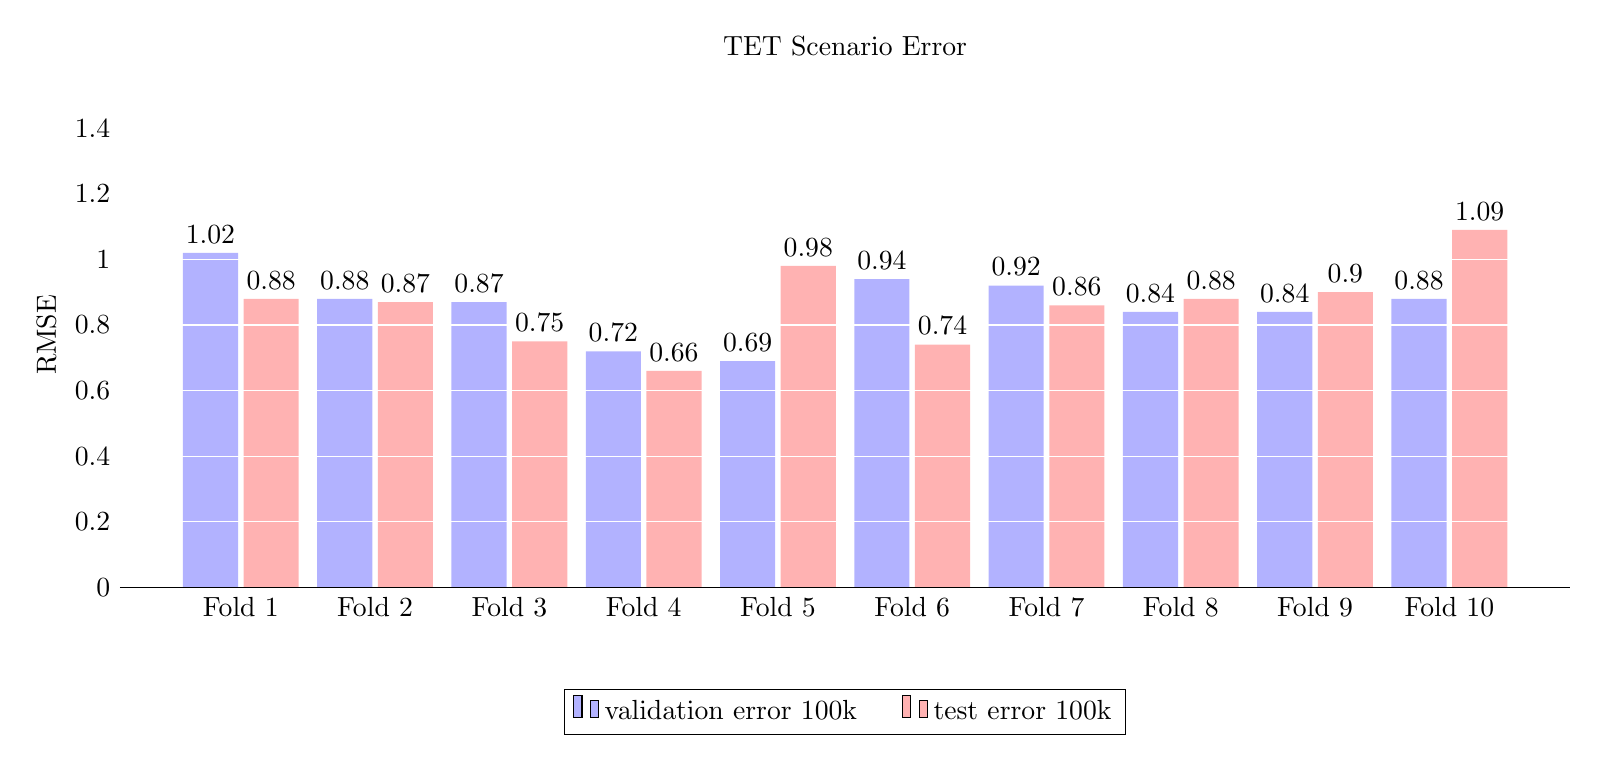
\begin{tikzpicture}
  \centering
  \begin{axis}[
        ybar, axis on top,
        title={TET Scenario Error},
        height=8cm, width=20cm,
        bar width=0.7cm,
        ymajorgrids, tick align=inside,
        major grid style={draw=white},
        enlarge y limits={value=.1,upper},
        ymin=0, ymax=1.4,
        axis x line*=bottom,
        y axis line style={opacity=0},
        tickwidth=0pt,
        enlarge x limits=true,
        legend style={
            at={(0.5,-0.2)},
            anchor=north,
            legend columns=-1,
            /tikz/every even column/.append style={column sep=0.5cm}
        },
        ylabel={RMSE},
        symbolic x coords={
           Fold 1,Fold 2,
           Fold 3,Fold 4,
           Fold 5,Fold 6,
           Fold 7,Fold 8,
           Fold 9,Fold 10},
       xtick=data,
       nodes near coords={
        \pgfmathprintnumber[precision=2]{\pgfplotspointmeta}
       }
    ]
    \addplot [draw=none, fill=blue!30] coordinates {
      (Fold 1, 1.02)
      (Fold 2, 0.88)
      (Fold 3, 0.87)
      (Fold 4, 0.72)
      (Fold 5, 0.69)
      (Fold 6, 0.94)
      (Fold 7, 0.92)
      (Fold 8, 0.84)
      (Fold 9, 0.84)
      (Fold 10, 0.88)};
   \addplot [draw=none,fill=red!30] coordinates {
      (Fold 1, 0.88)
      (Fold 2, 0.87)
      (Fold 3, 0.75)
      (Fold 4, 0.66)
      (Fold 5, 0.98)
      (Fold 6, 0.74)
      (Fold 7, 0.86)
      (Fold 8, 0.88)
      (Fold 9, 0.90)
      (Fold 10, 1.09)};
    \legend{validation error 100k, test error 100k}
  \end{axis}
  \end{tikzpicture}
	\end{adjustbox}
	\caption{TET scenario error from 100k dataset}
	\label{fig:tet_scenario_errors}
\end{figure}

From the $3$ figures including \autoref{fig:tet_scenario_errors} we can clearly see that the TET comparison and predictions.
With a average RMSE for the ratings at around 0.79, close to 0.15 points better than the average for node2vec.

Looking at the runtime of the different methods during the tests, we found the average time it takes to run pr. person.
Bruteforce had an average runtime of 0.18 seconds.
The node2vec had an average runtime of 0.005 seconds.
The TET comparisons had an average of 5.02 seconds.

Looking at the different runtimes we see that node2vec is fastest at making recommendations and that the TETs takes around 1000 times as long to make a recommendation.
A reason for this difference is that the node2vec model is trained and stored in memory, making it faster and easier to look up the vectors and compute the similarities.
The TET runtime could potentially be improved by pre-computing the values, implementing a matrix containing the similarities, so that you can look up the result instead of calculating them for each user in runtime.